
\documentclass[margin=0]{standalone}
\usepackage{tikz}
\usepackage{pgfplots,pgfplotstable}
\usepackage{amsmath,amsfonts,amssymb,xfrac,cancel}
\usepackage{xifthen}
\usepackage{ifthen}
\usepackage{xfp}
\usepackage{tikz-dimline}

\usetikzlibrary{arrows,arrows.meta,bending,calc,decorations,shadings,shadows,shapes,shapes.arrows,shapes.geometric,spy,patterns,backgrounds}
\usepgfplotslibrary{units,fillbetween,groupplots,colorbrewer,colormaps}
\pgfplotsset{compat=newest,
	axis line style={line width=0.8pt},
	every axis/.style = {
		scale only axis,
		width=7cm,height=5cm,
		tick style = {line width=0.8pt,black},
		ticklabel style={scale=0.85},
		major tick length = 1.5mm,
		minor tick length = 0.75mm,
		minor x tick num=1,
		minor y tick num=1,
		xlabel style={scale=1},
		ylabel style={scale=1},
		zlabel style={scale=1},
		%xlabel={Photon energy (eV)}, 
		%    	xticklabel style={
			%    	/pgf/number format/precision=2,
			%    	/pgf/number format/fixed,
			%    	/pgf/number format/fixed zerofill,
			%    },
		yticklabel style={
			/pgf/number format/precision=2,
			/pgf/number format/fixed,
			/pgf/number format/fixed zerofill,
		},
		xtick scale label code/.code={},
	},
	every axis plot/.style={smooth,line width=0.5pt},
	/pgfplots/legend image code/.code={%
		\draw[mark repeat=1,mark phase=1,#1] 
		plot coordinates {
			(0cm,0cm) 
			(0.0cm,0cm)
			(0.0cm,0cm)
			(0.0cm,0cm)
			(0.3cm,0cm)%
		};
	},
}
\pgfplotsset{every axis legend/.style={
		cells={anchor=center},
		inner xsep=1pt,
		inner ysep=1pt,
		nodes={scale=0.7,inner sep=2pt, transform shape},
		draw=none,
		at={(1,1)},
		anchor=north east,
	}
}



\pgfplotsset{rellenoa/.style={pattern=north west lines,pattern color=gray}}

\newcommand{\errorband}[5]{
	\pgfplotstableread[col sep=comma]{#1}\datatable
	\addplot [name path=pluserror,draw=none,no markers,forget plot]
	table [x={#2},y expr=\thisrowno{#3}] {\datatable};
	
	\addplot [name path=minuserror,draw=none,no markers,forget plot]
	table [x={#2},y expr=\thisrowno{#4}] {\datatable};
	
	\addplot [rellenoa,forget plot,opacity=#5]
	fill between[of=pluserror and minuserror];
	
}

\begin{document}
\begin{tikzpicture}
\begin{axis}[%
name=harrison,
xmin=0,xmax=55,
xtick pos=left,
ytick pos=left,
ylabel={Energy (eV)},
xlabel={Growth ($z-$) axis (nm)},
]

\addplot[no markers,smooth,tension=0] table [x index={0},y index={1},col sep=comma] {/media/labfiles/ruco/repos/cqws-codes/cqws-v1/first-codes/data/potential_profile.dat};

\addplot[no markers,smooth] table [x index={0},y expr=\thisrowno{1}*-1/20 + 0.04915,col sep=comma] {/media/labfiles/ruco/repos/cqws-codes/cqws-v1/first-codes/data/psielectron_data.dat};
\addplot[no markers,smooth,dashed] table [x index={0},y expr=\thisrowno{2}*-1/20 + 0.05772,col sep=comma] {/media/labfiles/ruco/repos/cqws-codes/cqws-v1/first-codes/data/psielectron_data.dat};


\end{axis}
\node[anchor=north west,inner sep=0mm,xshift=3mm](table) at (harrison.north east){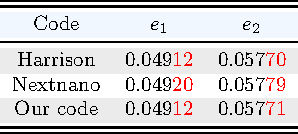
\includegraphics{../../../tables/table-comparison-numerical-results/out/comparison-numerical-harrison-nextnano.pdf}};
\node[draw, fill=blue,text=white,inner sep=0mm,font=\bfseries,scale=1.5] at (harrison.north west){a)};
\node[draw, fill=blue,text=white,inner sep=0mm,font=\bfseries,scale=1.5] at (table.north west){b)};

\end{tikzpicture}
\end{document}


